%
% コンピュータグラフィックスA レポート
%	(課題3回目)
%	門崎 雄紀, 22/1/27
%
\documentclass[12pt]{jreport}
\setlength{\textwidth}{160mm}
\setlength{\textheight}{230mm}
\setlength{\topmargin}{0mm}
\setlength{\oddsidemargin}{0mm}
\setlength{\evensidemargin}{0mm}
\usepackage[dvipdfmx]{graphicx}
\usepackage{tabverb}
\title{コンピュータグラフィックスA(担当教員: 乃万) \\ レポート(第3回)}
%%% 自分の履修科目名にあわせて1つだけ選択すること
\author{知能情報工学科 3年	\\ 192C1046 門崎雄紀}
%%% 自分の学科(大学院生は専攻・分野),学年,学生番号,氏名に書き換えること
\date{提出日: 2022 年 2 月 15 日}
%%% 実際の提出日に書き換えること
\begin{document}
\maketitle

\chapter{課題}
球を描け.

\section{プログラム}

以下に課題の内容を満たすプログラムを示す.
%%% プログラムリストは\begin{verbatim}から\end{verbatim}の間に書くこと
\begin{verbatim}
//
// sampleshade.c - シェーディングサンプルプログラム
//
#include <stdlib.h>
#include <stdio.h>
#include <GL/glut.h>
#include <math.h>

enum { VAO_0, NUM_VAO };	// 頂点配列オブジェクトの番号
enum { BUF_0, NUM_BUF };	// バッファオブジェクトの番号
enum { VERTLOC, NORMLOC };	// シェーダ属性位置の番号

// プリミティブの頂点の開始インデックスと個数
#define NUM_VERT_PLN	4
#define IDX_VERT_XYP	0
#define IDX_VERT_YZP	(IDX_VERT_XYP + NUM_VERT_PLN)
#define IDX_VERT_XYM	(IDX_VERT_YZP + NUM_VERT_PLN)
#define IDX_VERT_YZM	(IDX_VERT_XYM + NUM_VERT_PLN)
//#define NUM_VERT	(IDX_VERT_YZM + NUM_VERT_PLN)

#define NUM_DIV_THETA         15
#define NUM_DIV_PHY           15
#define NUM_VERT              NUM_DIV_PHY * (2 * (NUM_DIV_THETA + 1))

GLuint vao[NUM_VAO];	// 頂点配列オブジェクト
GLuint buf[NUM_BUF];	// バッファオブジェクト

GLuint program;		// プログラムオブジェクト

GLint uloc_pvmMatrix;	// ユニフォーム pvmMatrix 位置
GLint uloc_vmMatrix;	// ユニフォーム vmMatrix 位置
GLint uloc_lColor;	// ユニフォーム lColor 位置
GLint uloc_lDirection;	// ユニフォーム lDirection 位置
GLint uloc_ambColor;	// ユニフォーム ambColor 位置
GLint uloc_albDifAmb;	// ユニフォーム albDifAmb 位置
GLint uloc_albSpec;	// ユニフォーム albSpec 位置

#include "setup_shader.c"	// シェーダセット用関数
#include "nglmatrix.c"	// モダンOpenGL用互換行列計算用関数

//
// init - sampleshade の初期化
//
void
init(void)
{
    GLfloat vtnr[NUM_VERT][6];// 頂点座標/法線の配列
    float theta;
    float phy;
    float dphy = M_PI / NUM_DIV_PHY;
    int idx = 0;
    
    for(int j = 0;j < NUM_DIV_PHY;j++){
        for(int i = 0;i <= NUM_DIV_THETA;i++){
            theta = 2 * i * M_PI / NUM_DIV_THETA;
            phy = -M_PI / 2 + dphy * j;

            //X座標、法線
            vtnr[idx][0] = vtnr[idx][3] = sin(theta) * cos(phy);
            vtnr[idx + 1][0] = vtnr[idx + 1][3] = sin(theta) * cos(phy + dphy);
            //Z座標、法線
            vtnr[idx][2] = vtnr[idx][5] = cos(theta) * cos(phy);
            vtnr[idx + 1][2] = vtnr[idx + 1][5] = cos(theta) * cos(phy + dphy);
            //Y座標、法線
            vtnr[idx][1] = vtnr[idx][4] = sin(phy);
            vtnr[idx + 1][1] = vtnr[idx + 1][4] = sin(phy + dphy);
            idx += 2;
        }
    }

// 頂点配列オブジェクト/バッファオブジェクトの生成
    glGenVertexArrays(NUM_VAO, vao);
    glGenBuffers(NUM_BUF, buf);
// 頂点配列オブジェクト/バッファオブジェクトのバインド
    glBindVertexArray(vao[VAO_0]);
    glBindBuffer(GL_ARRAY_BUFFER, buf[BUF_0]);
// 頂点配列によるバッファオブジェクトの設定
    glBufferData(GL_ARRAY_BUFFER, sizeof(vtnr), vtnr, GL_STATIC_DRAW);
// 頂点/フラグメントシェーダのセットとプログラムオブジェクトの生成
    //program = setup_shader("gouraud.vert", "gouraud.frag");
	program = setup_shader("phong.vert", "phong.frag");
// ユニフォーム位置の検出
    uloc_pvmMatrix = glGetUniformLocation(program, "pvmMatrix");
    uloc_vmMatrix = glGetUniformLocation(program, "vmMatrix");
    uloc_lColor = glGetUniformLocation(program, "lColor");
    uloc_lDirection = glGetUniformLocation(program, "lDirection");
    uloc_ambColor = glGetUniformLocation(program, "ambColor");
    uloc_albDifAmb = glGetUniformLocation(program, "albDifAmb");
    uloc_albSpec = glGetUniformLocation(program, "albSpec");
#ifdef MYDEBUG
    fprintf(stderr, "uloc_pvmMatrix = %d\n", uloc_albSpec);
#endif

// 頂点属性関係の設定
    glVertexAttribPointer(VERTLOC, 3, GL_FLOAT, GL_FALSE,
     6 * sizeof(GLfloat), 0);
    glEnableVertexAttribArray(VERTLOC);
    glVertexAttribPointer(NORMLOC, 3, GL_FLOAT, GL_FALSE,
     6 * sizeof(GLfloat), (GLvoid *)(3 * sizeof(GLfloat)));
    glEnableVertexAttribArray(NORMLOC);
}

// ビューイングパラメータ
static float trns_z = 5.0;	// z方向の移動距離
static float rot_x = 30.0;	// x軸中心の回転角
static float rot_y = 20.0;	// y軸中心の回転角
static float vrp_x = 0.0;	// 参照視点のx座標
static float vrp_y = 0.0;	// 参照視点のy座標
static float vrp_z = 0.0;	// 参照視点のz座標
static float v_agl = 60.0;	// 縦方向の視野角
static float near = 1.0;	// 前方クリッピング面までの距離
static float far = 20.0;	// 後方クリッピング面までの距離

// 光源パラメータ
static GLfloat lCol[3] = { 3.0, 3.0, 3.0 };	// 光源色(RGB別強さ)
static GLfloat lDir[3] = { 1.0, 0.0, 0.0 };	// 光源方向(ワールド座標系)
static double light_rot = 0.0;			// 光源回転角(y軸回り)
static GLfloat ambCol[3] = { 0.2, 0.2, 0.2 };	// 環境光色(RGB別強さ)

static GLfloat proj[16];	// 投影行列

//
// display - 表示コールバック関数
//
void
display(void)
{
    GLfloat pvm[16];	// 投影/視野/モデリング変換行列
    GLfloat v[16];		// 視野変換行列
    GLfloat m[16];		// モデリング変換行列
    GLfloat vm[16];		// 視野/モデリング変換行列
    GLfloat difamb[3];	// 拡散/環境反射率
    GLfloat spec[2];	// 鏡面反射率とn
    GLfloat lDirRot[3];	// 回転後光源方向(ワールド座標系)
    GLfloat lDirv[3];	// 回転後光源方向(カメラ座標系)
    double light_rot_rad, sin_lrot, cos_lrot;	// 光源回転関係
    int i;

    glClear(GL_COLOR_BUFFER_BIT | GL_DEPTH_BUFFER_BIT); // 画面のクリア
// 頂点配列オブジェクトのバインド
    glBindVertexArray(vao[VAO_0]);
// 視野変換行列の設定
    nglLoadIdentity(v);
    nglTranslate(v, 0.0, 0.0, -trns_z);
    nglRotateX(v, rot_x);
    nglRotateY(v, rot_y);
    nglTranslate(v, -vrp_x, -vrp_y, -vrp_z);
// モデリング変換は恒等変換(ワールド座標系に直接描画)
    nglLoadIdentity(m);
// 視野/モデリング変換行列の設定
    nglLoadIdentity(vm);
    nglMultMatrix(vm, v);
    nglMultMatrix(vm, m);
    glUniformMatrix4fv(uloc_vmMatrix, 1, GL_FALSE, vm);
// 投影/視野/モデリング変換行列の設定
    nglLoadIdentity(pvm);
    nglMultMatrix(pvm, proj);
    nglMultMatrix(pvm, vm);
    glUniformMatrix4fv(uloc_pvmMatrix, 1, GL_FALSE, pvm);
// 光源の回転と光源パラメータの設定
    light_rot_rad = light_rot * M_PI / 180.0;
    sin_lrot = sin(light_rot_rad);
    cos_lrot = cos(light_rot_rad);
    lDirRot[0] = cos_lrot * lDir[0] + sin_lrot * lDir[2];
    lDirRot[1] = lDir[1];
    lDirRot[2] = - sin_lrot * lDir[0] + cos_lrot * lDir[2];
    // 光源方向をビューイング座標系に
    for (i = 0; i < 3; i++) {
	lDirv[i] = v[i] * lDirRot[0] + v[4 + i] * lDirRot[1]
	         + v[8 + i] * lDirRot[2];
    }
    glUniform3fv(uloc_lDirection, 1, lDirv);
    glUniform3fv(uloc_lColor, 1, lCol);
    glUniform3fv(uloc_ambColor, 1, ambCol);
// 反射率等の設定
    difamb[0] = 0.3; difamb[1] = 0.0; difamb[2] = 0.4;
    glUniform3fv(uloc_albDifAmb, 1, difamb);
    spec[0] = 1.0; spec[1] = 20.0;
    glUniform2fv(uloc_albSpec, 1, spec);
// 球体の描画
    for(int i = 0;i < NUM_DIV_PHY;i++){
        glDrawArrays(GL_TRIANGLE_STRIP, 2 * i * (NUM_DIV_THETA + 1), 2 * (NUM_DIV_THETA + 1));
    }

    glutSwapBuffers();
#ifdef MYDEBUG
    GLfloat v2[3];
    glGetUniformfv(program, uloc_albDifAmb, &v2);
    fprintf(stderr, "albDifAmb r %f g %f b %f\n", v2[0], v2[1], v2[2]);
    glGetUniformfv(program, uloc_albSpec, &v2);
    fprintf(stderr, "albSpec ks %f n %f\n", v2[0], v2[1]);
    GLfloat mat2[16];
    int i2;
    glGetUniformfv(program, uloc_pvmMatrix, &mat2);
    for (i2 = 0; i2 < 16; i2++) {
	fprintf(stderr, "%8.4f", mat2[i2]);
	if (i2 % 4 == 3) {
	    fprintf(stderr, "\n");
	}
    }
#endif
}

//
// reshape - 再作成コールバック関数
//
void reshape(int width, int height)
{
    glViewport(0, 0, width, height);	// ビューポートの設定
// 投影行列の計算
    nglLoadIdentity(proj);
    ngluPerspective(proj, v_agl, (double)width / height, near, far);
}
    
//
// lightmove - 光源の回転パラメータ操作
//
void lightmove(void)
{
    light_rot += 0.3;
    glutPostRedisplay();
}

//
// keyboard - キーボードコールバック関数
//
void keyboard(unsigned char key, int x, int y)
{
    switch(key) {
    case 'a':
	rot_y += 5;
	glutPostRedisplay();
	break;
    case 'd':
	rot_y -= 5;
	glutPostRedisplay();
	break;
    case 'w':
	rot_x += 5;
	glutPostRedisplay();
	break;
    case 's':
	rot_x -= 5;
	glutPostRedisplay();
	break;
    case 'L':
	light_rot += 5;
	glutPostRedisplay();
	break;
    case 'M':
	glutIdleFunc(lightmove);
	break;
    case 'm':
	glutIdleFunc(NULL);
	break;
    case 0x1b:	// ESC文字
	exit(0);
    }
}

//
// main - メイン関数
//
int
main(int argc, char** argv)
{
    glutInit(&argc, argv);		// GLUTの初期化
    glutInitDisplayMode(GLUT_DOUBLE | GLUT_RGBA | GLUT_DEPTH);
					// 表示モードの設定
    glutInitWindowSize(500, 500);	// ウィンドウサイズの設定
    glutCreateWindow("sampleshade");	// ウィンドウの生成

    printf("GL_VERSION : %s\n", glGetString(GL_VERSION));
					// OpenGLバージョンの表示
    init();				// 各種初期化
    // 各種コールバック関数の設定
    glutDisplayFunc(display);	// 表示コールバック関数の設定
    glutReshapeFunc(reshape);	// 再作成コールバック関数の設定
    glutKeyboardFunc(keyboard);	// キーボードコールバック関数の設定

    glEnable(GL_DEPTH_TEST);	// 陰面消去の指定
    glutMainLoop();

    return 0;
}

\end{verbatim}



\section{表示画像}
1.1章のプログラムを動作させると球体が表示される.グローシェーディングとフォンシェーディングの2つのシェーダで表示させた球体の画像を示す.

\begin{figure}
\begin{center}
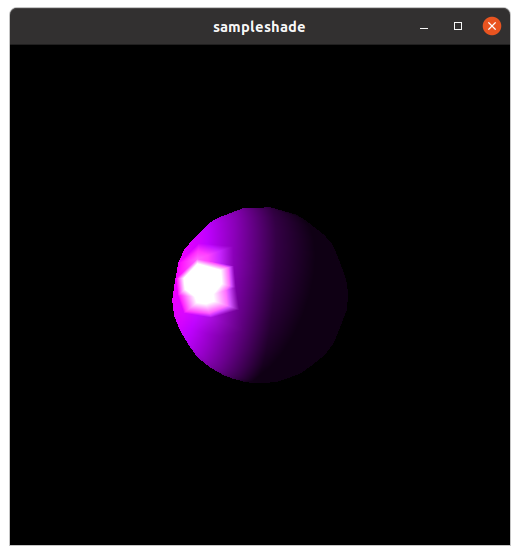
\includegraphics[width=70mm]{grourad.png}
\end{center}
\caption{グローシェーディングによる球体}

\begin{center}
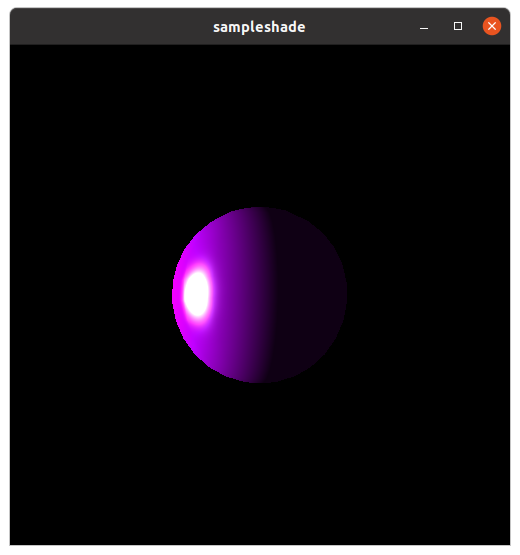
\includegraphics[width=70mm]{phong.png}
\end{center}
\caption{フォンシェーディングによる球体}

\end{figure}

\clearpage

\chapter{感想}
今回は球体の表示に挑戦した.頂点配列の外側にアクセスしてしまうなどのエラーに悩まされることもあったが、最終的にきれいに球体が表示できたので良かった.次は球体を複数表示し、衝突のアニメーションをさせるなどの発展的なプログラムを書きたいと思った.


\end{document}
